\section{Collected data} \label{apd:collection}

\begin{table}[h!]
    \centering
    \caption{Data and metadata collected.}% \raNote{Numbers may be slightly off -- double check}}
    \label{tab:data_collected}
    \resizebox{\columnwidth}{!}{
    \begin{tabular}{l|l}
		  \toprule
            Field & Description \\
			\midrule
			Reviews\\
			\midrule
			Content & Text of the review\\
			Author ID & Identifier is different for Recommended and not Recommend reviews\\
			Date & Date of posting\\
			Rating & Review rating \\
			Business ID & Identifier for the business the review was posted to\\
			Author data & Name and other public account information\\
			Recommended & Whether the review is Recommended\\
			\midrule
			Businesses\\
			\midrule
			Business ID & Identifier for the business\\
			Amenities & Listed amenities\\
			\bottomrule
    \end{tabular}
    }
\end{table}

\begin{figure}[h!]
    \centering
    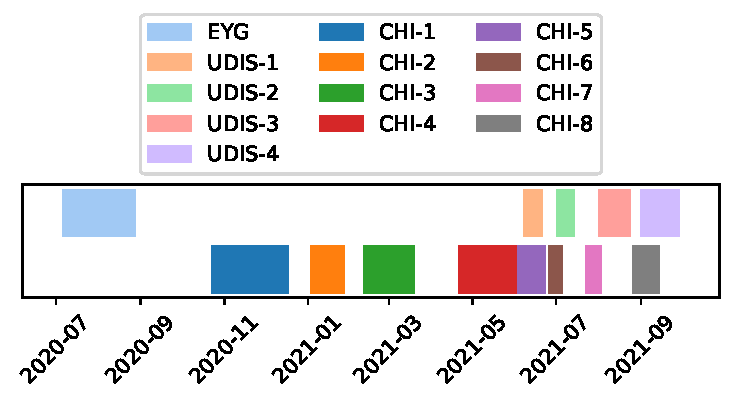
\includegraphics[width=0.9\columnwidth]{chapters/reviews/figures/crawl_timeline.pdf}
    \caption{The timeline for each crawl. Each box indicates the first and last operation for each crawl.}
    \label{fig:crawl_timeline}
\end{figure}

\begin{figure}[b!]
    \centering
    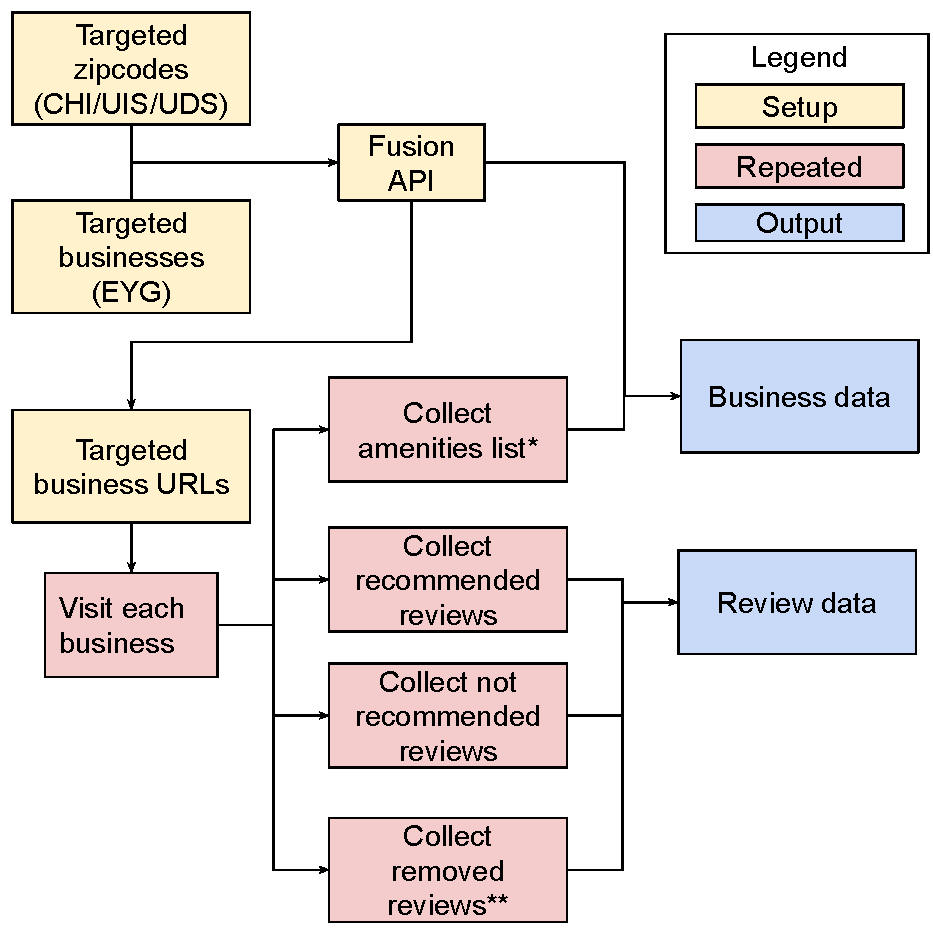
\includegraphics[width=0.9\columnwidth]{chapters/reviews/figures/Crawl diagram.pdf}
    \caption{The data collection process. Yellow indicates setup steps that are completed once. Red indicates steps that are completed for each timepoint. Blue indicates outputs.\\
    * Amenities were only collected for the CHI 8 and UDIS 4.\\
    ** Removed reviews were collected for CHI 7-8 and UDIS 3-4. }
    \label{fig:crawling_diagram}
\end{figure}
